
% Figure 4: Non-Uniform Voltage Grid + ΔV-Weighted Metric
% Compile: pdflatex fig4_voltage_grid.tex
\documentclass[border=4pt]{standalone}
\usepackage{tikz}
\usepackage{amsmath,amssymb}
\usepackage{pgfplots}
\pgfplotsset{compat=1.18}
\usetikzlibrary{arrows.meta,calc,decorations.pathreplacing}

% ── ICML Global Colour System ──
\definecolor{ink}{HTML}{1F2937}
\definecolor{flagship}{HTML}{2563EB}
\definecolor{secondary}{HTML}{D97706}
\definecolor{physgood}{HTML}{059669}
\definecolor{errbad}{HTML}{BE123C}
\definecolor{muted}{HTML}{64748B}
\definecolor{panelbg}{HTML}{F8FAFC}
\definecolor{gridline}{HTML}{E2E8F0}
\definecolor{mppgold}{HTML}{F59E0B}

\begin{document}
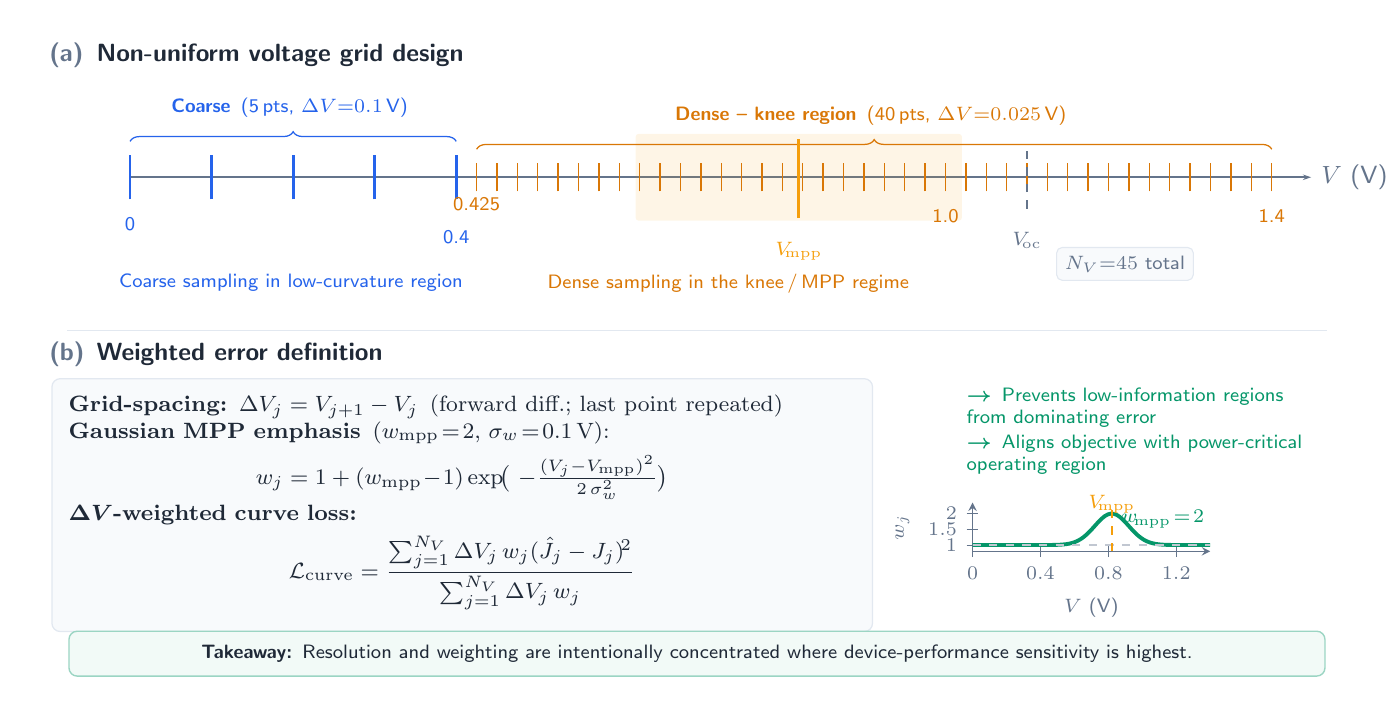
\begin{tikzpicture}[every node/.style={font=\sffamily,text=ink}]

% ── Canvas: 17.0 cm × 8.2 cm ──
\useasboundingbox (0,0) rectangle (17,8.2);

% ════════════════════════════════════════════════
%  PANEL (a)  -  Non-uniform voltage grid design
% ════════════════════════════════════════════════
\node[font=\sffamily\small\bfseries,text=muted,anchor=west]
  at (0.15,7.85) {(a)};
\node[font=\sffamily\small\bfseries,anchor=west]
  at (0.75,7.85) {Non-uniform voltage grid design};

% ── Axis geometry ──
\pgfmathsetmacro{\axL}{1.3}           % left end (cm)
\pgfmathsetmacro{\axR}{15.8}          % right end (cm)
\pgfmathsetmacro{\axY}{6.30}          % axis y-position
\pgfmathsetmacro{\vs}{(\axR-\axL)/1.4}% cm per volt

% Horizontal voltage axis
\draw[-{Stealth[length=3pt,width=2pt]},line width=0.7pt,muted]
  (\axL,\axY) -- (\axR+0.5,\axY)
  node[right,font=\sffamily\small,text=muted]{$V$ (V)};

% ── MPP highlight zone (light alpha fill) ──
\fill[mppgold,opacity=0.10,rounded corners=1pt]
  ({\axL+0.62*\vs},{\axY-0.55})
  rectangle ({\axL+1.02*\vs},{\axY+0.55});

% ── Coarse ticks: 0-0.4 V, ΔV = 0.1 V, 5 pts ──
\foreach \v in {0.0,0.1,0.2,0.3,0.4}{
  \pgfmathsetmacro{\xp}{\axL+\v*\vs}
  \draw[flagship,line width=1.0pt]
    (\xp,{\axY-0.28}) -- (\xp,{\axY+0.28});
}
\node[below=3pt,font=\sffamily\scriptsize,text=flagship]
  at (\axL,{\axY-0.28}) {0};
\node[below=8pt,font=\sffamily\scriptsize,text=flagship]
  at ({\axL+0.4*\vs},{\axY-0.28}) {0.4};

% Coarse brace - single-line spec
\draw[decorate,decoration={brace,amplitude=3.5pt,raise=5pt},
  line width=0.45pt,flagship]
  (\axL,{\axY+0.28}) -- ({\axL+0.4*\vs},{\axY+0.28})
  node[midway,above=10pt,font=\sffamily\scriptsize,text=flagship,
       align=center]{
    \textbf{Coarse}\enspace(5\,pts, $\Delta V{=}0.1$\,V)
  };

% ── Dense ticks: 0.425-1.4 V, ΔV = 0.025 V, 40 pts ──
\foreach \i in {0,1,...,39}{
  \pgfmathsetmacro{\v}{0.425+\i*0.025}
  \pgfmathsetmacro{\xp}{\axL+\v*\vs}
  \draw[secondary,line width=0.5pt]
    (\xp,{\axY-0.18}) -- (\xp,{\axY+0.18});
}
\node[below=1pt,font=\sffamily\scriptsize,text=secondary]
  at ({\axL+0.425*\vs},{\axY-0.10}) {0.425};
\node[below=3pt,font=\sffamily\scriptsize,text=secondary]
  at ({\axL+1.0*\vs},{\axY-0.18}) {1.0};
\node[below=3pt,font=\sffamily\scriptsize,text=secondary]
  at ({\axL+1.4*\vs},{\axY-0.18}) {1.4};

% Dense brace - single-line spec
\draw[decorate,decoration={brace,amplitude=3.5pt,raise=5pt},
  line width=0.45pt,secondary]
  ({\axL+0.425*\vs},{\axY+0.18}) -- ({\axL+1.4*\vs},{\axY+0.18})
  node[midway,above=10pt,font=\sffamily\scriptsize,text=secondary,
       align=center]{
    \textbf{Dense -- knee region}\enspace
    (40\,pts, $\Delta V{=}0.025$\,V)
  };

% ── Vmpp marker (label below to avoid brace overlap) ──
\pgfmathsetmacro{\xmpp}{\axL+0.82*\vs}
\draw[mppgold,line width=1.2pt]
  (\xmpp,{\axY-0.52}) -- (\xmpp,{\axY+0.48});
\node[below=5pt,font=\sffamily\scriptsize\bfseries,text=mppgold]
  at (\xmpp,{\axY-0.52}) {$V_{\!\mathrm{mpp}}$};

% ── Voc marker ──
\pgfmathsetmacro{\xvoc}{\axL+1.1*\vs}
\draw[muted,line width=0.6pt,dashed]
  (\xvoc,{\axY-0.40}) -- (\xvoc,{\axY+0.38});
\node[below=5pt,font=\sffamily\scriptsize,text=muted]
  at (\xvoc,{\axY-0.40}) {$V_{\!\mathrm{oc}}$};

% ── Required annotation callouts (colour-coded, below axis) ──
\node[font=\sffamily\scriptsize,text=flagship,anchor=north east]
  at ({\axL+0.42*\vs},{\axY-1.10})
  {Coarse sampling in low-curvature region};
\node[font=\sffamily\scriptsize,text=secondary,anchor=north west]
  at ({\axL+0.50*\vs},{\axY-1.10})
  {Dense sampling in the knee\,/\,MPP regime};

% Total-point badge
\node[draw=gridline,fill=panelbg,rounded corners=2pt,
  font=\sffamily\scriptsize,text=muted,inner sep=3pt]
  at ({\axL+1.22*\vs},{\axY-1.10})
  {$N_V{=}45$ total};

% ── Subtle panel separator ──
\draw[gridline,line width=0.35pt] (0.5,4.35) -- (16.5,4.35);

% ════════════════════════════════════════════════
%  PANEL (b)  -  Weighted error definition
% ════════════════════════════════════════════════
\node[font=\sffamily\small\bfseries,text=muted,anchor=west]
  at (0.15,4.05) {(b)};
\node[font=\sffamily\small\bfseries,anchor=west]
  at (0.75,4.05) {Weighted error definition};

% ── Equation card (compact, left column) ──
\node[
  draw=gridline,fill=panelbg,rounded corners=3pt,
  line width=0.45pt,
  text width=10.0cm,align=left,
  font=\footnotesize,text=ink,
  inner sep=6pt,anchor=north west,
] (eqnbox) at (0.3,3.75) {%
  \begingroup
  \abovedisplayskip=3pt
  \belowdisplayskip=1pt
  \abovedisplayshortskip=2pt
  \belowdisplayshortskip=1pt
  %
  \textbf{Grid-spacing:}
  $\Delta V_j = V_{j+1} - V_j$%
  \enspace(forward diff.; last point repeated)%
  \par%
  \textbf{Gaussian MPP emphasis}%
  \enspace($w_{\mathrm{mpp}}\!=\!2$, $\sigma_w\!=\!0.1$\,V):%
  \[
    w_j =  1 + (w_{\mathrm{mpp}}\!-\!1)
    \exp\!\bigl(\
    -\tfrac{(V_j - V_{\mathrm{mpp}})^{2}}{2\,\sigma_w^{2}}
    \bigr)
  \]%
  \textbf{$\boldsymbol{\Delta V}$-weighted curve loss:}%
  \[
    \mathcal{L}_{\mathrm{curve}}
    = 
    \frac{%
      \textstyle\sum_{j=1}^{N_V}
      \Delta V_j \, w_j 
      (\hat{J}_j - J_j)^{\!2}
    }{%
      \textstyle\sum_{j=1}^{N_V}
      \Delta V_j \, w_j
    }
  \]%
  \endgroup
};

% ── Right column: annotation callouts ──
\node[font=\sffamily\scriptsize,text=physgood,
  anchor=north west,text width=4.4cm,align=left]
  at (11.8,3.75) {%
    $\boldsymbol{\rightarrow}$\enspace
    Prevents low-information regions
    from dominating error%
  };
\node[font=\sffamily\scriptsize,text=physgood,
  anchor=north west,text width=4.4cm,align=left]
  at (11.8,3.15) {%
    $\boldsymbol{\rightarrow}$\enspace
    Aligns objective with
    power-critical operating region%
  };

% ── Right column: mini Gaussian-weight plot ──
\begin{scope}[shift={(12.0,1.55)}]
  \begin{axis}[
    width=4.6cm,height=2.2cm,
    at={(0,0)},anchor=south west,
    xlabel={$V$ (V)},ylabel={$w_j$},
    xlabel style={font=\sffamily\scriptsize,text=muted},
    ylabel style={font=\sffamily\scriptsize,text=muted},
    tick label style={font=\sffamily\scriptsize,text=muted},
    xmin=0,xmax=1.4,ymin=0.8,ymax=2.35,
    axis lines=left,
    axis line style={line width=0.35pt,color=muted},
    every tick/.style={muted,line width=0.25pt},
    xtick={0,0.4,0.8,1.2},
    ytick={1.0,1.5,2.0},
    grid=none,clip=false,
  ]
    \addplot[physgood,line width=1.4pt,smooth,samples=80,domain=0:1.4]
      {1.0 + 1.0*exp(-((x-0.82)^2)/(2*0.1^2))};
    \addplot[muted!40,line width=0.4pt,dashed,domain=0:1.4] {1.0};
    \draw[mppgold,line width=0.6pt,dashed]
      (axis cs:0.82,0.8) -- (axis cs:0.82,2.15);
    \node[font=\sffamily\scriptsize,text=mppgold]
      at (axis cs:0.82,2.30) {$V_{\!\mathrm{mpp}}$};
    \node[font=\sffamily\scriptsize,text=physgood]
      at (axis cs:1.12,1.82) {$w_{\!\mathrm{mpp}}\!=\!2$};
  \end{axis}
\end{scope}

% ════════════════════════════════════════════════
%  TAKEAWAY CALLOUT
% ════════════════════════════════════════════════
\node[
  draw=physgood!40,fill=physgood!5,
  rounded corners=3pt,line width=0.50pt,
  font=\sffamily\scriptsize,text=ink,
  inner sep=5pt,text width=15.6cm,align=center,
] at (8.5,0.25) {%
  \textbf{Takeaway:}\enspace
  Resolution and weighting are intentionally concentrated
  where device-performance sensitivity is highest.%
};

\end{tikzpicture}
\end{document}
